\documentclass[11pt]{article}
\usepackage[utf8]{inputenc}
\usepackage[czech]{babel}
\usepackage[utf8]{inputenc}
\usepackage{times}
\usepackage{graphicx}
\usepackage[a4paper,top=30mm,left=20mm,textwidth=17cm,textheight=24cm]{geometry}
\usepackage{hyperref}
\usepackage{enumitem}

\begin{document}

    \begin{titlepage}
        \begin{center}
            
\includegraphics[width=1\linewidth]{fit logo.png} \\
            
            \vspace{\stretch{0.382}}
            
            \Huge{Dokumentace projektu IFJ} \\ 
            \LARGE{Implementace překladače imperativního jazyka IFJ21} \\
            \Large{Tým 027, varianta 1} \\
            \Large{[BOOLTHEN, FUNEXP, OPERATORS]}
            
            \vspace{\stretch{0.618}}
        \end{center}
        \hfill
        \begin{center}
        \LARGE
            \begin{tabular}{l  l  l}
                \textbf{Vojtěch Dvořák} & \textbf{xdvora3o} & \; xx\% \\
                 Tomáš Dvořák & xdvora3r & \; xx\% \\
                 Juraj Dedič &  xdedic07 & \; xx\% \\
                 Radek Marek & xmarek77 & \; xx\%
            \end{tabular}
        \end{center}
    \end{titlepage}
    
    %%%%%%%%%%%%%%%%%%%%%%%%%%%%%%%%%%%%%%%%%%%%%%%%%%%%%%%%%%%
    \setcounter{page}{1}
    \tableofcontents
    \clearpage
    %%%%%%%%%%%%%%%%%%%%%%%%%%%%%%%%%%%%%%%%%%%%%%%%%%%%%%%%%%%
    \section{Úvod}
        Cílem projektu bylo vytvořit překladač v~jazyce C, který zpracuje kód ze zdrojového jazyka IFJ21 (podmnožinou jazyka Teal) a následně jej přeloží do cílového jazyka IFJcode21. \\
    	\indent Program načte vstup ze standartního vstupu, zanalyzuje a v~případě, že načtený kód neobsahuje žádné chyby, vygeneruje výsledný kód. V~opačném případě ukončí provádění a vrátí chybový kód odpovídající typu chyby.
    \vspace{10mm}
	\section{Implementace}
	
	\subsection{Lexikální analýza}
    	Náš lexikální analyzátor je řízen konečným automatem, který je implementován pomocí tabulky přechodových funkcí (staticky alokované pole). Stavy konečného automatu jsou identifikovány k~tomu určeným výčtovým datovým a tyto identifikátory zároveň představují index zmíněné tabulky. \\
    	\indent Přechodovými funkcemi označujeme funkce, které obsahují množství podmínek, na základě, kterých se rozhoduje, do kterého stavu se automat přepne, případně zda má analyzátor vrátit token s~příslušných typem. \\
     	\indent Token v~našem analyzátoru vyznačuje strukturu obsahující typ, atribut a index, který ukazuje na  určité místo v~bufferu, v~němž jsou uloženy hodnoty všech tokenů, vyjma těch předdefinovaných (klíčová slova, oddělovače, operátory). Ty jsou uloženy ve speciálních statických polích kvůli lepšímu hospodaření s~alokovanou pamětí. Pokud během lexikální analýzy dojde k~chybě, automat vrátí token s~chybovým typem. 

	\subsection{Syntaktická analýza}
	    Syntaktický analyzátor získává tokeny prostřednictví lexikálnáho analyzátoru a na základě typu a atributu rozhoduje které z~gramatických pravidel použije, nebo zda se jedná o~syntaktickou chybu. Zároveň však probíhá kontrola, zda typ tokenu není chybný, v~tomto případě vrátí lexikální chybu. \\
	    \indent V~případě, že syntaktický analyzátor dorazí na místo, kde očekává výraz, předá řízení přecedenčnímu syntaktickému analyzátoru. Ten následně výraz redukuje pomocí pravidel uložených ve staticky alokovaném poli a ní tabulky. \\
	    \indent Z~možností v~zadání jsme vybrali implementaci pomocí rekurzivního sestupu.
	
	\subsection{Sémantická analýza}
    	Souběžně se syntaktickou analýzou probíhá sémantická analýza. Ke kontrole se používá zejména tabulka symbolu společně s~návratovými hodnotami precedenčního syntaktického analyzátoru. Při kontrole datových typů ve zdrojovém kódu (jazyce) používáme speciální výčtový datový typ a znaky uložené v~dynamicky alokovaných řetězcích, které identifikují datové typy a jejich počet. Toto nám umožňuje snadno provádět tyto typové kontroly pří mnohonásobném přiřazení, nebo funkcí s~více než jednou návratovou hodnotou. \\
    	\indent V~případě aritmetických, řetězcových a relačních výrazů	 analyzátor kontroluje typovou kompatibilitu na základě staticky alokované tabulky, ve které se nachází popis možných datových typů pro zpracovávanou operaci. Při redukci, je výsledný typ operace propagován do struktury vzniklého neterminálu.
    	
        \pagebreak
        
	\subsection{Generování kódu}
	    Generování probíhá opět souběžně se syntaktickou a sémantickou analýzou. Veškeré vestavěné funkce jsou vygenerovány na začátku každého kódu, ať už jsou použité nebo ne, bez vědomí uživatele. \\
	    \indent Pro volání funkcí, vyhodnocování výrazů a návratové hodnoty využíváme výhradně zásobník a dočasný rámec. Při volání funkcí využíváme zásobník rámců pro zanořování. Při práci s~proměnnými najdeme unikátní identifikátor v~tabulce symbolů. Kontrola běhových chyb je vyřešena pomocí předdefinovaných funkcí, převážně na hodnotu NIL a dělení nulou. \\
	    \indent Před vytisknutím programu v~cílovém jazyce na standartní výstup je vytvořena vnitřní reprezentace pomocí \hyperref[sec:dll]{dvojsměrně vázaného seznamu}. 
	    
	\vspace{5mm}
    \section{Datové struktury}
    
    \subsection{Binární vyhledávací strom}
        Tuto strukturu využíváme, jak nám ukládá zadání, pro implementaci tabulky symbolů. Kromě základní struktury a operací jsme implementovali možnost zřetězit více BVS. Zřetězení jsme dosáhli využitím přítomností indexů nadřazeného bloku, který je uložen v~dynamickém poli. Toho využíváme při hledání proměnných v~nadřazených blocích kódu.\\
        Při iplementaci jsme vycházeli z~našich řešení projektů do předmětu IAL.
    
    \subsection{Dynamické pole}
        Vyjma staticky alokovaných polí, využity například pro snadnou implementaci precedenční tabulky, tabulky vestavěných funkci nebo tabulku klíčových slov, náš překladač také využívá dynamicky alokovaná pole. \\
        \indent Rozhodli jsmme se pro tuto možnost hlavně z~důvodů teoreticky neomezené kapacity a spojitého uložení dat v~paměti, lze tak jednoduše vypisovat v~nich uložené řetězce pomocí standartních funkcí. Náročné realokace při zvětšování nejsou tak podstatné, protože náš systém není real-time aplikací.
    
    \subsection{Zásobník}
        Zásobník hraje naprosto zásadní roli v~precedenčním syntaktickém analyzátoru při zpracování veškerých výrazu. Struktura se však osvědčila i v~jiných částech našeho
        překladače. \\
        \indent Příkladem je vyhodnocování mnohonásobných přiřazovacích operací, kde se
        jednotlivé prvky přiřazují směrem z~prava do leva. V~tomto případě jsou do zásobníku
        ukládány ukazatele na sekvence instrukcí v~cílovém jazyce, které jednotlivé výrazy
        reprezentují. Následně se zásovník vyprázdňuje jsou napojovány na hlavní tělo
        generovaného programu. \\
        \indent Náš zásobník je implementován prostřednictvím dynamicky alokoveného pole,
        umožnuje realokaci a následné zvětšení kapacity v~případě potřeby. Pro snadnější a
        čístší implementaci jsme si zavedli makro, které dokáže snadno vygenerovat tuto
        strukturu pro různé datové typy, což výrazně snižuje redundanci kódu.
        
    \subsection{Dvojsměrně vázaný seznam}
    \label{sec:dll}

        Strukturu využíváme pro uložení instrukcí cílového jazyka před jejich vypsáním na
        standartní výstup. Každá položka obsahuje dynamický řetězec s~zpravidla jednou
        instrukcí a odkazy na předchozí a následující instrukci. Tato reprezentace umožňuje
        cílový kód takřka libovolně editovat v~průběhu překladu, tato vlastnost je důležitý
        zejména při deklarací proměnných hodnot uvnitř těla cyklu. \\
        \indent Díky dvojsměrně vázanému seznamu si můžeme uchovávat ukazaten před začátkem
        cyklu, kam postupně vkládáme deklarace v~cílovém jazyce, ty by uvniř cyklu mohly
        způsopbit chybu z~důvodů redeklarace proměnných.
        
    \section{Členění implementačního řešení}
        \begin{tabular}{l l}
            Lexikální analyzátor & \; \verb|scanner.{c,h}| \\
            Syntaktický analyzátor & \; \verb|parser_topdown.{c,h}| \\ 
            Precedenční analyzátor & \; \verb|precedentparser.{c,h}| \\
            Sémantický analyzátor & \; \verb|parser_topdown.{c,h}| \\
            Generování kódu & \; \verb|generator.{c,h}|
        \end{tabular}
    \vspace{10mm}
    \section{Práce v~týmu}
    
    \subsection{Rozdělení práce}
        \begin{tabular}{l  l}
                \textbf{Vojtěch Dvořák} & Vedení týmu, organizace, dohlížení nad repozitářem, kontrola,             precedenční analýza  \\
                        & lexikální analýza, sémantická analýza\\
                Tomáš Dvořák & generování kódu   \\
                Juraj Dedič & syntaktická analýza, generování kódu \\
                Radek Marek & testování, dokumentace, prezentace, lehká sémantická analýza 
        \end{tabular}
    
    \subsection{Verzovací systém}
        Jako verzovací systém jsme si vybrali Git a vzdálený repozitář na serveru GitHub. \\
    	\indent Tento výběr nám dovolil pracovat zároveň na více částech programu najednou. Každý člen týmu pracoval ve vlastním odvětví a při určitých intervalech se všechna naše řešení spojili do jednoho. 

    \subsection{Komunikace}
        Komunikace probíhala převážně přes Discord, kde jsme využívaly textové a hlasové místnosti a připínání důležitých věcí a událostí. \\
    	\indent Pravidelně jsme se scházeli jednou týdne, ale s~blížícím se datem odevzdání se počet setkání zvyšoval. 
    	
	
    
    %%%%%%%%%%%%%%%%%%%%%%%%%%%%%%%%%%%%%%%%%%%%%%%%%%%%%%%%%%%
    
    \section{Diagram konečného automatu}
        \vspace{9mm}
        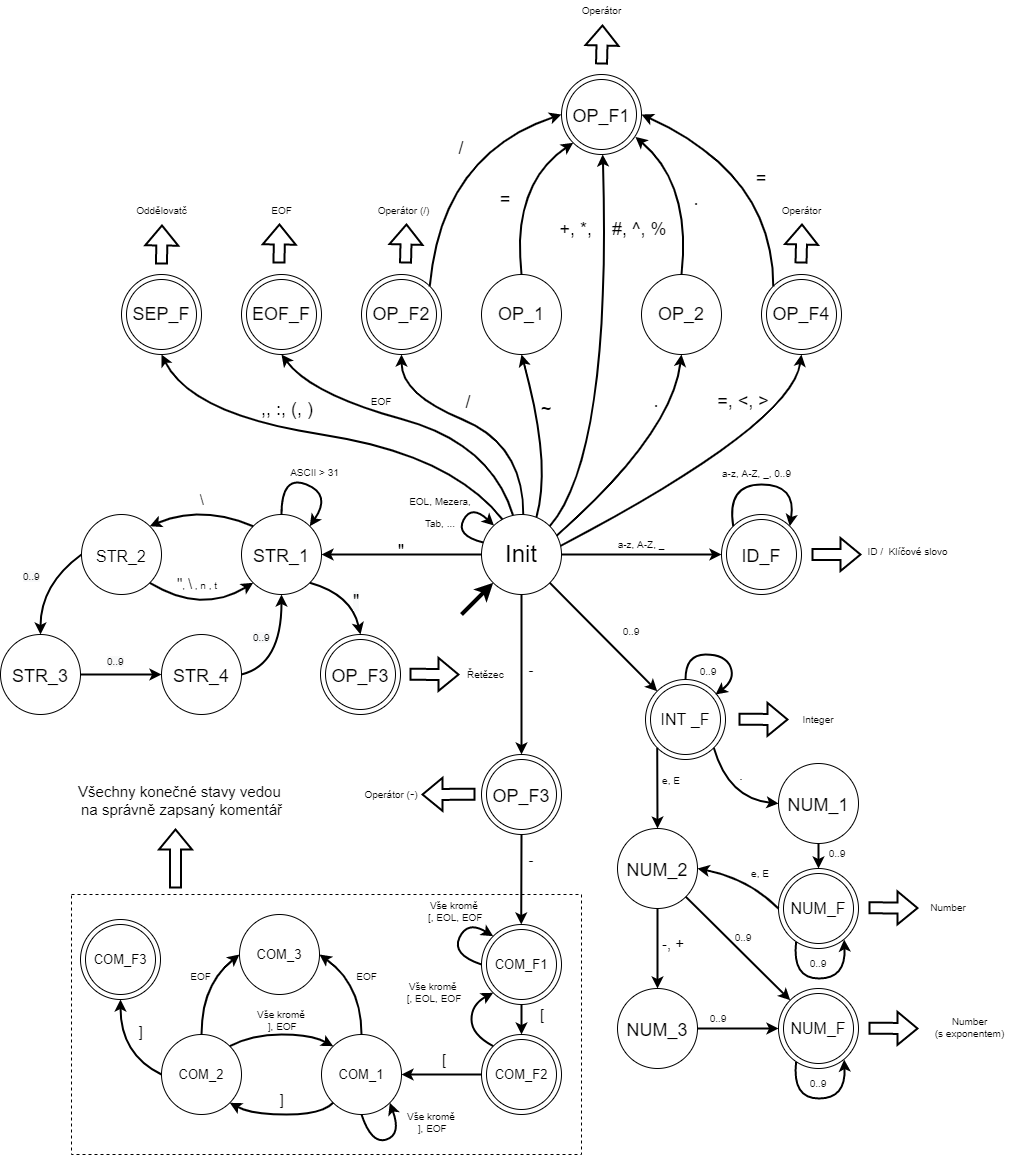
\includegraphics[width=1\linewidth]{FSM.png}
        \pagebreak
    
    %%%%%%%%%%%%%%%%%%%%%%%%%%%%%%%%%%%%%%%%%%%%%%%%%%%%%%%%%%%
    
    \section{LL -- Gramatika}
        \begin{enumerate}[noitemsep]
            \normalsize
            \item\verb|program               ::= prolog global-statement-list|
            \item\verb|prolog                ::= require"ifj21"|
            \item\verb|statement-list        ::= statement statement-list|
            \item\verb|statement-list        ::= |$\varepsilon$
            \item\verb|global-statement      ::= global[id]:function( decl-param-list ) type-list|
            \item\verb|decl-param-list       ::= [type] decl-param|
            \item\verb|decl-param-list       ::= |$\varepsilon$
            \item\verb|decl-param            ::= ,[type]|
            \item\verb|decl-param            ::= |$\varepsilon$
            \item\verb|statement             ::= local[id]:[type] value-assignment|
            \item\verb|value-assignment      ::= |$\varepsilon$
            \item\verb|value-assignment      ::= = expression|
            \item\verb|statement             ::= function-call| 
            \item\verb|statement             ::= assignment| 
            \item\verb|assignment            ::= id-list = expression-list| 
            \item\verb|id-list               ::=  [id] id-list-1| 
            \item\verb|id-list-1             ::= ,[id] id-list-1| 
            \item\verb|id-list-1             ::= |$\varepsilon$ 
            \item\verb|statement             ::= if expression then statement-list else-branch end| 
            \item\verb|else-branch           ::= |$\varepsilon$ 
            \item\verb|else-branch           ::= else statement-list| 
            \item\verb|statement             ::= while expression do statement-list end| 
            \item\verb|global-statement      ::= function-call| 
            \item\verb|argument-list         ::= argument argument-list-1| 
            \item\verb|argument-list         ::= |$\varepsilon$ 
            \item\verb|argument-list-1       ::= , argument argument-list-1| 
            \item\verb|argument-list-1       ::= |$\varepsilon$ 
            \item\verb|argument              ::= expression| 
            \item\verb|function-call         ::= [function-id]( argument-list  )| 
            \item\verb|global-statement-list ::= global-statement global-statement-list| 
            \item\verb|global-statement ::= function[id](param-list) type-list statement-list end| 
            \item\verb|function-type-def     ::= |$\varepsilon$ 
            \item\verb|function-type-def     ::= type-list| 
            \item\verb|param-list            ::= [id]:[type] param-list-1| 
            \item\verb|param-list-1          ::= ,[id]:[type] param-list-1| 
            \item\verb|param-list-1          ::= |$\varepsilon$ 
            \item\verb|type-list             ::= |$\varepsilon$ 
            \item\verb|type-list             ::= :[type] type-list-1| 
            \item\verb|type-list-1           ::= ,[type] type-list-1| 
            \item\verb|type-list-1           ::= |$\varepsilon$ 
            \item\verb|statement             ::= return expression-list| 
            \item\verb|expression-list       ::=  expression expression-list-1| 
            \item\verb|expression-list       ::= |$\varepsilon$ 
            \item\verb|expression-list-1     ::= , expression expression-list-1| 
            \item\verb|expression-list-1     ::= |$\varepsilon$  \end{enumerate}
            \pagebreak
    %%%%%%%%%%%%%%%%%%%%%%%%%%%%%%%%%%%%%%%%%%%%%%%%%%%%%%%%%%%
  
    \section{LL -- Tabulka}
        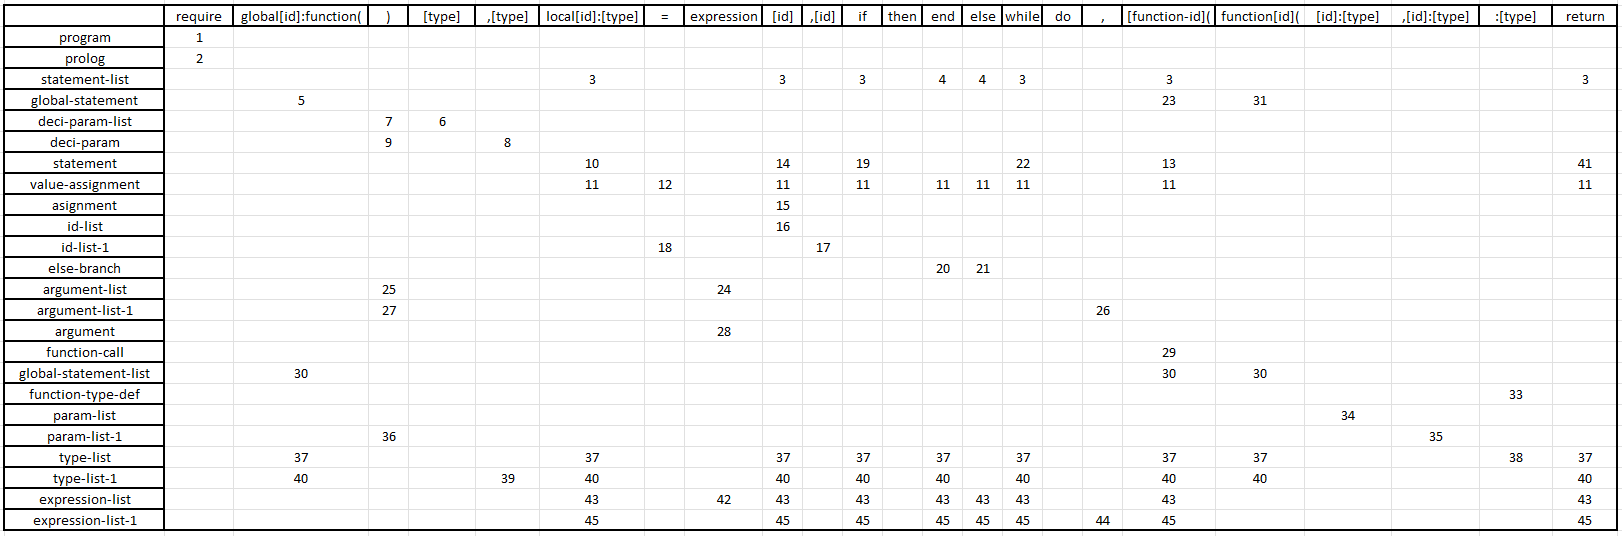
\includegraphics[width=1\linewidth]{lltable.png}
        
    \vspace{15mm}
    
    \section{Precedenční tabulka}
        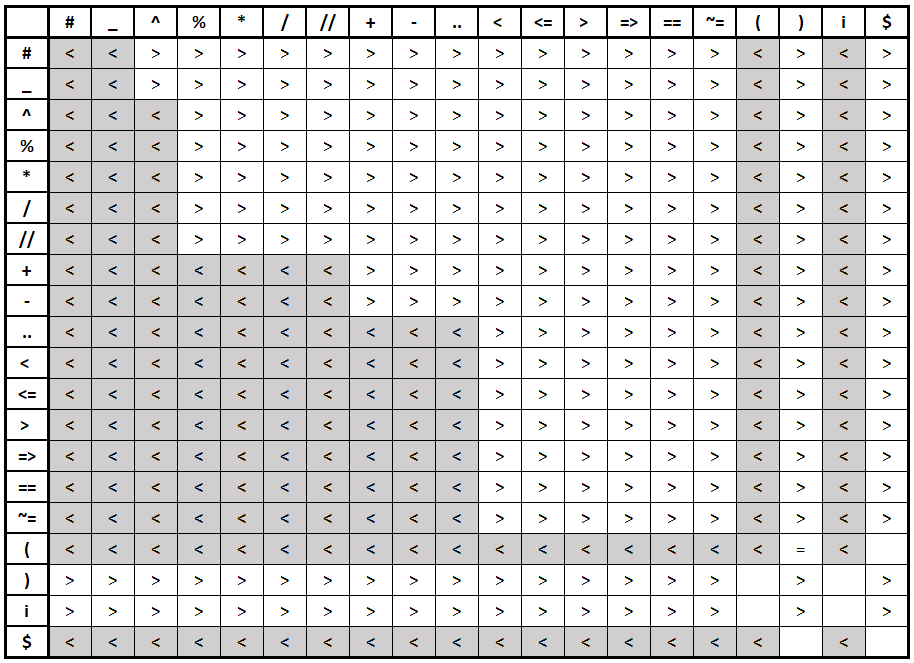
\includegraphics[width=1\linewidth]{precedencni tabulka.png}
        \pagebreak
\end{document}
